\documentclass[14pt,UTF-8,a4paper,titlepage]{ctexbook}
\usepackage[left=3cm,right=3cm,top=3cm,bottom=3cm]{geometry}
\usepackage{graphicx}
\usepackage[colorlinks]{hyperref}
\usepackage{listings}
\usepackage{draftwatermark} %水印包
\SetWatermarkText{贝尔加教育} %水印的标示
\SetWatermarkLightness{0.8} %水印的亮度
\SetWatermarkScale{0.7}      %水印的大小
\usepackage{pgf,tikz,pgfplots}
\pgfplotsset{compat=1.5}
\usepackage{mathrsfs}
\usetikzlibrary{arrows}
\title{\zihao{1}贝尔加初中数学讲义}
\author{陈应洪}
\date{\today}
\begin{document}
\maketitle
\tableofcontents
\chapter{ 初中数学思想和解题方法}
\paragraph{思考:现在有一个空水壶、水、煤气灶、火机,让你烧一壶水你怎么烧?如果其他条件不变,只是水壶里面有半壶开水,让你烧一壶开水,你怎么做?}.\par
(1)数形结合法:数学家华罗庚说得好:“数形结合百般好,隔离分家万事休,几何代数统一体,永远联系莫分离”.几何图形的形象直观,便于理解,代数方法的一般性,解题过程的机械化,可操作性强,便于把握,因此数形结合思想是数学中重要的思想方法.所谓数形结合就是根据数学问题的题设和结论之间的内在联系,既分析其数量关系,又揭示其几何意义使数量关系和几何图形巧妙地结合起来,并充分地利用这种结合,探求解决问题的思路,使问题得以解决的思考方法.每个几何图形中蕴含着一定的数量关系,而数量关系常常又通过图形的直观性作出反映和描述,数与形之间可以相互转化,将问题化难为易,化抽象为具体. 数形结合的思想方法通过借数解形、以形助数,能使某些较复杂的数学问题迎刃而解.\par
(2)分类讨论法:在数学中,我们常常需要根据研究对象性质的差异,分各种不同情况予以考查.这种分类思考的方法是一种重要的数学思想方法,同时也是一种解题策略.分
类是按照数学对象的相同点和差异点,将数学对象区分为不同种类的思想方法,掌握分类的方法,领会其实质,对于加深基础知识的理解.提高分析问题、解决问题的能力是十分
重要的.正确的分类必须是周全的,既不重复、也不遗漏.分类的原则:(1)分类中的每一部分是相互独立的;(2)一次分类按一个标准;(3)分讨论应逐级进行.\par
(3)转化化归思想:所谓化归思想就是化未知为已知、化繁为简、化难为易.如将分式方程化为整式方程,将代数问题化为几何问题,将四边形问题转化为三角形问题等.实现
这种转化的方法有:待定系数法、配方法、整体代人法以及化动为静、由抽象到具体等.\par
(4)方程与函数思想:方程与函数是研究数量关系的重要工具,在处理某些问题时,往往根据已知与未知之间的内在联系和相等关系建立方程(或方程组)或函数关系,这种通
过方程(组)或函数来沟通已知与未知,从而使问题获得解决的思想方法称之为方程与函数思想.\par

\section{数型结合}
\setlength{\parindent}{0pt} 1、绝对值小于3的非负整数是,绝对值不大于4的整数是\rule[-5pt]{1.3cm}{0.05em}.\\
2、设$a>0$,$b<0$且$|a|<|b|$,用“<”号a,-a,b,-b把它们连接起来\rule[-5pt]{1.3cm}{0.05em}.\\
3、化简三个数a,b,c在数轴上的对应点如图1,化简$|a+b|-|b|+|a+c|-|c-a|$.\\
\begin{figure}[htb]
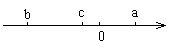
\includegraphics[scale=1]{1.jpg}
\caption{}
\end{figure}
4、化简$|a+c|+|b+c|-|a-b|$.\\
5、化简$|a-b|-|b+c|+|c-a|-|a+c|$.\\
6、若a,b为有理数,有$a>0,b<0,a+b$,比较$a,-a,-b,b$大小.\\
7、已知两数,a,b,如果a比b大,那么$|a|,|b|$的大小\rule[-5pt]{1.3cm}{0.05em}.\\
8、用数轴方程解方程.\\
\qquad \qquad (1)、$|x+5|+2=5$ \qquad\qquad\qquad\qquad\qquad\qquad (2)、$|x-3|-3=2$\par
\vspace{5cm}
9、$|x-1|+|x-3|$的最小值.(注:绝对值是指一个数在数轴上所对应点到原点的距离,用“||”表示.|b-a|或者|a-b|表示数轴上表示a点到b点的距离).\\
10、先阅读下面的材料,然后解答问题:\\
\hspace{16pt} 在一条直线上有依次排列的n(n>1)台机床在工作,我们要设置零件供应站P,使这n台机床到供应站P的距离总和最小,要解决这个问题,先退到比较简单的情形:\\
\hspace{16pt}如图,如果直线上有2台机床时,很明显设在A1和A2之间的任何地方都行,因为甲和乙走的距离之和等于A1到A2的距离.\par
\hspace{16pt}如图②,如果直线上有3台机床时,不难判断,供应站设在中间一台机床A2处最合适,因为如果P放在A2处,甲乙和丙所走的距离之和恰好为A1到A3的距离,而如果把P放到别处,例如D处,那么甲和丙所走的距离之和仍是A1到A3的距离,可是乙还得走从A2到D的这一段,在是多出来的,一次P放在A2处是最佳选择.不难知道,如果直线上有4台机床,P应设在第2台与第3台之间的任何地方;有5台机床,P应设在第3台的位置.\par
问题1:有n台机床时,P应设置在何处?\par
\vspace{3cm}
问题2:根据问题1的结论,求$|x-1|+|x-2|+|x-3|+|x-4|+|x-5|+.....+|x-617|$的最小值.
\vspace{4cm}
\section{分类讨论}
1、解不等式方程.\\
\qquad \qquad (1)、$|x+5|+2=5$ \qquad\qquad\qquad\qquad\qquad\qquad (2)、$|x-3|-3=2$\par
\vspace{3cm}
2、已知a、b互为相反数,c、d互为倒数,x的平方是4,求$x^2-(a+b+cd)x+(a+b)^{2008}+(-cd)^{2009}$的值.\par
\vspace{3cm}
3、已知a为有理数且$a \neq 0 $,则$\frac{a}{|a|}+\frac{2|a|}{a}$= \rule[-5pt]{1.3cm}{0.05em}.\par
4、已知a,b均为不等于0的有理数,则代数$\frac{|a|}{a}+\frac{b}{|b|}+\frac{ab}{|ab|} $的值为\rule[-5pt]{1.3cm}{0.05em}.\par
5、求代数式$\frac{a}{|a|}+\frac{b}{|b|}+\frac{ab}{|ab|} $的值为 \rule[-5pt]{1.3cm}{0.05em}.\par
6、若$abc\neq 0 $,$\frac{a}{|a|}+\frac{2b}{|2b|}+\frac{3c}{|3c|} $.\rule[-5pt]{1.3cm}{0.05em}.\par
7、解关于x的方程:\\
$(a-x)x=b-1$\\
\vspace{3cm}
\section{整体带入法}
1、$(\frac{1}{2}+\frac{1}{3}+\frac{1}{4}...\frac{1}{1999})(1+\frac{1}{2}+\frac{1}{3}+\frac{1}{4}...\frac{1}{1998})-(1+\frac{1}{2}+\frac{1}{3}+\frac{1}{4}...\frac{1}{1999})(\frac{1}{2}+\frac{1}{3}+\frac{1}{4}...\frac{1}{1998})$\par
\vspace{2cm}
2、求$(1-\frac{1}{2^2} )(1-\frac{1}{3^2} )(1-\frac{1}{4^2} )(1-\frac{1}{5^2} )...(1-\frac{1}{2018^2} )$\par
\vspace{2cm}
3、$(\frac{1}{2}+\frac{1}{3}+\frac{1}{4}...\frac{1}{2008})(1+\frac{1}{2}+\frac{1}{3}+\frac{1}{4}...\frac{1}{2007})-(1+\frac{1}{2}+\frac{1}{3}+\frac{1}{4}...\frac{1}{2008})(\frac{1}{2}+\frac{1}{3}+\frac{1}{4}...\frac{1}{2007})$\\
\chapter{勾股定理}
\section{勾股定理各种题型}
\subsection{方程思想和勾股定理结合的题目}
1、一旗杆在其$\frac{1}{3} $的B处折断,量得AC=5米,则旗杆原来的高度为(   ).\\
\begin{figure}[h]
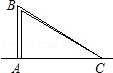
\includegraphics[scale=1]{2.jpg}
\end{figure}
A.$\sqrt{5}$米 \hfill B.$2\sqrt{5}$米 \hfill  C.10米 \hfill  D.$5\sqrt{3}$米\par
2、如图,在$\delta $ ABC中,$\angle$ B=40°,EF$//$AB,$\angle$1=$50^{\circ}$,CE=3,EF比CF大1,则EF的长为( ).\\
\begin{figure}[h]
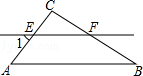
\includegraphics[scale=1]{3.jpg}
\end{figure}
A.5 \hfill B.6 \hfill  C.3 \hfill  D.4\par
3、已知,如图长方形ABCD中,AB=3cm,AD=9cm,将此长方形折叠,使点B与D重合,折痕为EF,则BE的长为().\\
\begin{figure}[h]
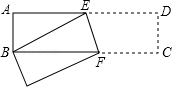
\includegraphics[scale=1]{4.jpg}
\end{figure}
A.3cm \hfill B.4cm \hfill  C.5cm \hfill  D.6cm \par
4、在我国古代数学著作《九章算术》中记载了一个有趣的问题,这个问题的意思是:有一个水池,水面是一个边长为10尺的正方形,在水池正中央有一根新生的芦苇,它高出水面1尺,如图所示,如果把这根芦苇垂直拉向岸边,它的顶端恰好到达岸边的水面.那么水深多少?芦苇长为多少?\par
\begin{figure}[h]
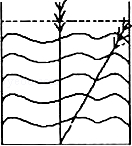
\includegraphics[scale=0.6]{5.jpg}
\end{figure}
\subsection{求最短距离问题}
1、如图,长方体的底面边长为~1~cm和~3~cm,高为~6~cm.如果用一根细线从点A开始经过4个侧面缠绕一圈到达~B,那么所用细线最短需要(  )\\
A.12cm \hfill B.11cm \hfill  C.10cm  \hfill  D.9cm \par  
\begin{figure}[h]
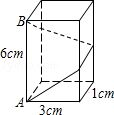
\includegraphics[scale=1]{6.jpg}
\end{figure}
2、如图,是一长、宽都是3cm,高BC=9cm的长方体纸箱,BC上有一点P,$pC=\frac{2}{3}BC$,一只蚂蚁从点A出发沿纸箱表面爬行到点P的最短距离是(  )\\
A.$6\sqrt{2}$cm \hfill B.$3\sqrt{3}$ cm \hfill  C.10cm \hfill  D.12cm \par
\begin{figure}[h]
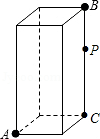
\includegraphics[scale=1]{7.jpg}
\end{figure}
3.如图,小红想用一条彩带缠绕易拉罐,正好从A点绕到正上方B点共四圈,已知易拉罐底面周长是12cm,高是20cm,那么所需彩带最短的是(  )\\
A.$13$cm \hfill B.$4\sqrt{61}$ cm \hfill  C.$4\sqrt{34}$cm \hfill  D.52cm \par 
\vspace{0.2cm}

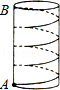
\includegraphics[scale=1.2]{8.jpg} \hspace{1cm}
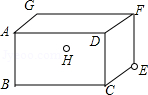
\includegraphics[scale=1.2]{10.jpg}  \hspace{1cm}
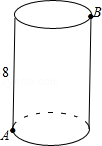
\includegraphics[scale=0.8]{11.jpg}\par
4.长方体敞口玻璃罐,长、宽、高分别为16cm、6cm和6cm,在罐内点E处有一小块饼干碎末,此时一只蚂蚁正好在罐外壁,在长方形ABCD中心的正上方2cm处,则蚂蚁到达饼干的最短距离是多少cm.(  )\\
A.$7\sqrt{5}$cm \hfill B.$\sqrt{233}$ cm \hfill  C.24cm  \hfill  D.$\sqrt{232}$cm \par

5.如图,一圆柱高8cm,底面半径为$\frac{6}{\pi}$cm,一只蚂蚁从点A爬到点B处吃食,要爬行的最短路程是().
\subsection{网格问题}
1.1、在边长为1的小正方形组成的网格中,$\bigtriangleup$ABC的三个顶点均在格点上,则$\bigtriangleup$ABC中BC边上的高为
\begin{figure}[h]
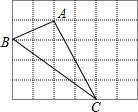
\includegraphics[scale=1]{12.jpg}
\end{figure}
2.如图,方格纸中每个小方格都是边长为1的正方形,我们把以格点连线为边的多边形称为“格点多边形”.如图(一)中四边形ABCD就是一个“格点四边形”.\\
(1)求图中四边形ABCD的面积;\\
(2)在图方格纸中画一个格点三角形EFG,使$\bigtriangleup$EFG的面积等于四边形ABCD的面积且为轴对称图形.\par
\chapter{全等三角形}
\section{全等三角形}
\subsection{学习要求}
1.理解全等图形及全等三角形的概念,能识别全等三角形中的对应边,对应角.\\
2.掌握全等三角形的表示方法及全等三角形的性质.\\
3.通过平移、翻折和旋转一个三角形等活动,发展、感知两个全等三角形的特征,学会判断对应的元素的方法.\\
\subsection{概念}
\textbf{1.全等的概念}:能够完全重合的两个图形叫做全等形(全等形关注的是两个图形的形状和大小,判断两个图形是否全等两个图形是否可以重合在一起).\\
\textbf{2.三角形的概念}:能够完全重合的两个三角形形叫做全三角形.\\
\textbf{3.对应元素}:把两个全等三角形的重合在一起,重合的顶点叫作对应顶点,重合的边叫作对应边,重合的角叫作对应角.\\
\textbf{例} 如图,已知$\bigtriangleup      ABC \cong \bigtriangleup DEC$写出所有的对应边,对应角.\\
\definecolor{ffffff}{rgb}{1.,1.,1.}
\begin{tikzpicture}[line cap=round,line join=round,>=triangle 45,x=1.0cm,y=1.0cm]
\clip(-5.199904850177654,-1.1965600451285707) rectangle (2.870913519509735,2.972193095388202);
\fill[line width=2.pt,,color=ffffff] (-4.,0.) -- (2.,0.) -- (0.,2.) -- cycle;
\fill[line width=2.pt,color=ffffff] (-4.464101615137754,2.2679491924311224) -- (0.7320508075688775,-0.7320508075688772) -- (0.,2.) -- cycle;
\draw [line width=1.2pt,] (-4.,0.)-- (2.,0.);
\draw [line width=1.2pt,] (2.,0.)-- (0.,2.);
\draw [line width=1.2pt,] (0.,2.)-- (-4.,0.);
\draw [line width=1.2pt] (-4.464101615137754,2.2679491924311224)-- (0.7320508075688775,-0.7320508075688772);
\draw [line width=1.2pt] (0.7320508075688775,-0.7320508075688772)-- (0.,2.);
\draw [line width=1.2pt] (0.,2.)-- (-4.464101615137754,2.2679491924311224);
\begin{scriptsize}
\draw [fill=black] (-4.,0.) circle (0.5pt);
\draw[color=black] (-4.013845454980116,-0.1824441717200292) node {$\LARGE{A}$};
\draw [fill=black] (2.,0.) circle (0.5pt);
\draw[color=black] (2.23928425579507,0.07020753376583584) node {$\LARGE{B}$};
\draw [fill=black] (0.,2.) circle (0.5pt);
\draw[color=black] (0.2391249206986299,2.070366868862267) node {$\LARGE{C}$};
\draw[color=black] (-1.346966341518196,-0.13331745120888877) node {$\LARGE{c}$};
\draw[color=black] (1.3058765660833977,0.8913255765948971) node {$\LARGE{a}$};
\draw[color=black] (-2.385645575182312,1.3264479582649982) node {$\LARGE{b}$};
\draw [fill=black] (-4.464101615137754,2.2679491924311224) circle (0.5pt);
\draw[color=black] (-4.2594790575358195,2.41425391244025) node {$\LARGE{A'}$};
\draw [fill=black] (0.7320508075688775,-0.7320508075688772) circle (0.5pt);
\draw[color=black] (0.9900619342260653,-0.6596751709711075) node {$\LARGE{B'}$};
\draw[color=black] (-1.1785318711942854,0.5965652535280546) node {$\LARGE{c'}$};
\draw[color=black] (0.5268671408353107,0.9334341941758746) node {$\LARGE{a'}$};
\draw[color=black] (-1.9996499140233501,2.3089823684878064) node {$\LARGE{b'}$};
\end{scriptsize}
\end{tikzpicture} \\
\textbf{4.表示方法}:全等用符号“$\cong$”表示,读作“全等于”.$\bigtriangleup      ABC \cong \bigtriangleup DEF$和表示$\bigtriangleup ABC$和$\bigtriangleup DEF$全等,读作"$\bigtriangleup ABC$全等于$\bigtriangleup DEF$". \\
\textbf{4.全等三角形的性质:}全等三角形的对应边相等;全等三角形的对应角相等.\\
\textbf{例}.如图,点$A,B,C,D$在同一条直线上,$\bigtriangleup ABF \cong  \bigtriangleup DCE$,$AF$和$DE$,$BF$和$CE$是对应边,求证:$AF//DE$\\
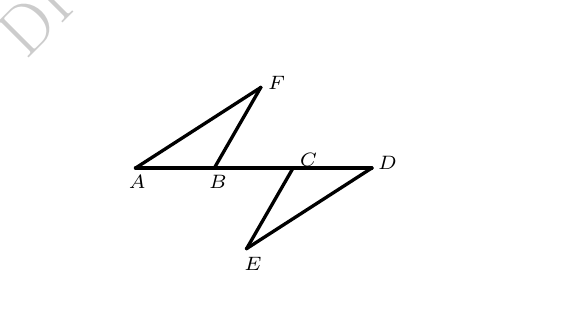
\begin{tikzpicture}[line cap=round,line join=round,>=triangle 45,x=1.0cm,y=1.0cm]
\clip(-1.370559629844417,-1.628276358312839) rectangle (5.322854646928852,1.7824547427211959);
\draw [line width=1.2pt] (2.,0.)-- (1.4107855359693817,-1.0227878702292361);
\draw [line width=1.2pt] (1.4107855359693817,-1.0227878702292361)-- (3.,0.);
\draw [line width=1.2pt] (3.,0.)-- (0.,0.);
\draw [line width=1.2pt] (0.,0.)-- (1.589214464030618,1.022787870229236);
\draw [line width=1.2pt] (1.589214464030618,1.022787870229236)-- (1.,0.);
\begin{scriptsize}
\draw [fill=black] (0.,0.) circle (0.5pt);
\draw[color=black] (0.02050646767628886,-0.17609647826507152) node {$\LARGE{A}$};
\draw [fill=black] (1.,0.) circle (0.5pt);
\draw[color=black] (1.0448898700346327,-0.18191683850574394) node {$\LARGE{B}$};
\draw [fill=black] (2.,0.) circle (0.5pt);
\draw[color=black] (2.1973211976877693,0.10328081328720436) node {$\LARGE{C}$};
\draw [fill=black] (3.,0.) circle (0.5pt);
\draw[color=black] (3.198423159083424,0.06253829160249746) node {$\LARGE{D}$};
\draw [fill=black] (1.4107855359693817,-1.0227878702292361) circle (0.5pt);
\draw[color=black] (1.4930576085664082,-1.2121206011047612) node {$\LARGE{E}$};
\draw [fill=black] (1.589214464030618,1.022787870229236) circle (0.5pt);
\draw[color=black] (1.789895980840701,1.08110133372017) node {$\LARGE{F}$};
\end{scriptsize}
\end{tikzpicture}

\chapter{一元二次方程}
\section{概念}
\subsection{定义}
只含有一个未知数,未知数的最高次数是~2,且系数不为~0,这样的方程叫一元二次方程.
\subsection{一般形式}
一元二次方程的一般形式为$ax^2+bx+c=0$($a$,$b$,$c$是已知数$a\neq 0 $).其中$a$,$b$,$c$分别叫做二次项系数、一次项系数、常数项.\par
(1)二次项、二次项系数、一次项、一次项系数,常数项都包括它前面的符号.\par
(2)要准确找出一个一元二次方程的二次项系数、一次项系数和常数项,必须把它先化为一般形式.\par
(3)形如$ax^2+bx+c=0$不一定是一元二次方程,当且仅当$a\neq 0$时是一元二次方程。\par
\subsection{判断一元二次方程}
一元二次方程必须同时满足以下三点:(1)方程是整式方程.(2)它只含有一个未知数.(3)未知数的最高次数是(同时还要注意在判断时,需将方程化成一般形式).
\section{解方程}
\textbf{1.直接开平方法:}对形如$(x+a)^2=b(b\geq 0)$的方程两边直接开平方而转化为两个一元一次方程的方法. \par 
(1)$9x^2-16=0$ \hspace{1cm}(2)$(x+5)^2-16=0$ \hspace{1cm}(3)$(x-5)^2=(3x+1)$  \\
\vspace{2cm}

\textbf{2.配方法1:}解一元二次方程时,在方程的左边加上一次项系数一半的平方,再减去这个数,使得含未知数的项在一个完全平方式里,这种方法叫做配方,配方后就可以用因式分解法或直接开平方法了,这样解一元二次方程的方法叫做配方法(\textbf{注意}:用配方法解一元二次方程$x^2+px+q=0$,当对方程的左边配方时,一定记住在方程的左边加上一次项系数的一半的平方后,还要再减去这个数).\\
(1)$x^2+6x-5=0$\hspace{1cm} (2)$x^2-\frac{7}{2}-2=0$\\
\vspace{2cm}

\textbf{3.配方法2:}当一元二次方程的形式为$ax^2+bx+c=0(a\neq 0,a\neq 1 )$时,用配方法解一元二次方程的步骤:(1)先把二次项的系数化为1:方程的左、右两边同时除以二项的系数;(2) 移项:在方程的左边加上一次项系数的一半的平方,再减去这个数,把原方程化为$(x+m)^2=n $的形式;
(3)若$n\geq 0 $,用直接开平方法或因式分解法解变形后的方程。\\
(1)$3x^2-9x+2=0 $  \hspace{3cm}  (2)$-x^2-4x+3=0$\\
\vspace{2cm}

\textbf{4.求根公式法:}一元二次方程$ax^2+bx+c=0(a\neq 0 ) $的求根公式是:$x=\frac{-b\pm \sqrt{b^2-4ac} }{2a} $
用求根公式法解一元二次方程的步骤是:(1)把方程化为$ax^2+bx+c=0(a\neq 0) $的形式,确定的值$a,b,c $(注意符号);(2)求出$b^2-4ac $的值;(3)若$b^2-4ac\geq 0$ ,则a,b把及$b^2-4ac $的值代人求根公式,求出 $x=\frac{-b\pm \sqrt{b^2-4ac} }{2a} $,求出$x_1,x_2$.\\
(1)$2x^2-3x-1=0$ \hfill  (2)$2x(x+\sqrt{2})+1=0$ \hfill  (3)$x^2+x+25=0$\\
\vspace{3cm}

\textbf{5.因式分解法:} 把方程左边的多项式(方程右边为0时)的公因式提出,将多项式写出因式的乘积形式,然后利用“若$pq=0$时,则$p=0$或$q=0$”来解一元二次方程的方法,称为因式分解法。\\
(1)$x^2-5x+6=0$  \hfill  (2)$x^2-x-12=0$\par
\vspace{2cm}

(3)$x^2-4x+3=0$ \hfill (4)$2x^2-3x-5=0$\par
\vspace{2cm}

\textbf{列}选方法解方程:\\
(1)$(2x-3)^2=9(2x+3)^2$ \hfill (2)$x^2-8x+6=0$ \hfill  (3)$(x+2)(x-1)=0$
\vspace{2cm}

\section{一元二次方程根的判别式} 
(1)$\bigtriangleup =b^2-4ac >0 \longmapsto $ 方程有两个不相等的实数根.\\
(2)$\bigtriangleup =b^2-4ac =0 \longmapsto $
方程有两个相等的实数根.\\
(3)$\bigtriangleup =b^2-4ac <0 \longmapsto $
方程有无实数根.\\
\textbf{列} 判断下列一元二次方程根的情况:\\
(1)$2x^2-3x-5=0 $\hfill (2)$9x^2=30x-25 $\hfill (3)$x^2+6x+10=0$\\
\vspace{2cm}

\textbf{例:} $m$为何时,方程$(2m+1)x^2+4mx+2m-3=0$的根满足下列情况:\\
(1)有两个不相等的实数根;\hfill (2)有两个不相等的实数根;\hfill (3)没有实数根;\\
\vspace{2cm}

\section{根与系数的关系}
若$x_1,x_2$是一元二次方程$ax^2+bx+c=0(a\neq 0 )$的两个根,则有,$x_1+x_2=-\frac{b}{a},x_1x_2=\frac{c}{a} $根据一元二次方程的根与系数的关系求值常用的转化关系:\\
${x_1}^2+{x_2}^2=(x_1+x_2)^2-2x_1x_2$ \\
$(x_1-x_2)^2=(x_1+x_2)^2-4x_1x_2$\\
${x_1}^2\cdot x_2+x_1\cdot {x_2}^2=x_1\cdot x_2(x_1+x_2)$ \\
$(x_1+a)(x_2)=x_1\cdot x_2+a(x_1+x_2)+a^2$ \\
$\frac{1}{x_1}+\frac{1}{x_2}=\frac{x_1+x_2}{x_1\cdot x_2}$ \\
$\frac{1}{{x_1}^2}+\frac{1}{{x_2}^2}=\frac{{x_1}^2+{x_2}^2}{{x_1}^2\cdot {x_2}^2}=\frac{(x_1+x_2)^2-2x_1x_2}{(x_1\cdot x_2)^2}$ \\
$|x_1-x_2|=\sqrt{(x_1-x_2)^2}=\sqrt{(x_1+x_2)^2-4x_1 x_2}$ \\
\textbf{例}:已知方程$2x^2-5x-3=0$的两根为$x_1,x_2$,不解方程,求下列各式的值.\par
(1)${x_1}^2+{x_2}^2$ \hspace{5cm} (2)$(x_1-x_2)^2$
\section{习题}
\subsection{定义}
1.关于$x$的一元二次方程$(k-1)x^2-2x+1=0$有两个不相等的实数根,则实数$k$的取值范围是.\par
2.已知关于x的一元二次方程$x^2+x+m^2-2m=0$有一个实数根为-1,求m的值及方程的另一实根.
3.将下列方程化为一般形式,并分别指出它们的二次项系数、一次项系数和常数项.

(1)$(x-2)(x+3)=8$  \hspace{3cm}    (2)$(3x-4)(x+3)=(x+2)^2$\\
\vspace{2cm}

4.已知关于$x$的方程$(m-1)x^{m^2+2}-(m+1)x-2=0$是一元二次方程时,则$m$= \\
5.关于x的方程$(k+1)x^2+3(k-2)x+k^2-42=0$的一次项系数是-6,则$k$=\\
\subsection{解一元二次方程}
1.用配方法解一元二次方程$x^2-6x-4=0$,下列变形正确的是\\
A.$(x-6)^2=-4+36$\hfill B.$(x-6)^2=4+36$\hfill C.$(x-3)^2=-4+9$\hfill D.$(x-3)^2=4+9$ \hfill  

2.若方程$x^2-x=0$的两个根为$x_1,x_2(x_1<x_2)$,则$x_2-x_1$=

3.方程$x^3-x=0$的解是

4.方程$(2x+1)(x-1)=8(9-x)-1$的根为

5.用合适的方法解方程:\\
$x(x-2)+x-2=0$  \hspace{2cm}   $2x^2-7x-2=0$ \hspace{2cm}  $2(x-1)^2+5(x-1)+2=0$\\
\vspace{2cm}

$\sqrt{2x^2-9x+5}=x-3 $  \hspace{2cm}  $x^3-2x^2-3x=0$  \hspace{2cm} \\ 

\subsection{根与系数的关系}
1.已知关于x的一元二次方程$x^2+mx-8=0$的一个实数根为2,则另一实数根及m的值分别为\\
A.4,-2  \hfill   B.-4,-2  \hfill  C.4,2 \hfill D.-4,2\par
2.设$x_1,x_2$是方程$x^2+5x-3=0$的两根,则${x_2}^2+{x_2}^2$的值是\\
A.19 \hfill  B.25   \hfill  C.31  \hfill  D.30  \par

3、若$x_1,x_2$是一元二次方程$x^2-2x-1=0$的两个根,则${x_1}^2-x_1+x_2$的值为\\
A.-1 \hfill B.0      \hfill     C.2  \hfill      D.3 \par
4.已知关于x的一元二次方程$x^2+mx+n=0$的两个实数根分别为$x_1=-2,x_2=4$,则m+n的值是\\
 	A.-10 \hfill B.10 \hfill	C.-6	\hfill D.2  \par
5.设$x_1,x_2$是方程$2x^2+14x-16=0$的两个实数根,则$\frac{x_2}{x_1}+\frac{x_1}{x_2} $的值为\par
6.设$a,b$,是方程$x^2+x-2013=0$的两个不相等的实数根,$a^2+2a+b$的值\\
7.已知一元二次方程$x^2+3x+1=0$的两个根为$x_1,x_2$ 那么$(1+x_1)(1+x_2)$的值等于\\
8.已知为$x_1,x_2$ 是方程$x^2-3x+1=0$的两个实数根,则$\frac{1}{x_1}+\frac{1}{x_2} $的值是\\
9.关于$x$的一元二次方程$x^2+(2k+1)x+k^2+1=0$有两个不等实根$x_1,x_2$.\\
(1)求实数$k$的取值范围.\\
\vspace{2cm}

(2)若方程两实根$x_1,x_2$ 满足$|x_1|+|x_2|=x_1•x_2$,求k的值\\
\vspace{2cm}

\subsection{根的判别式}
1.一元二次方程$(x+1)^2-2(x-1)^2=7$的根的情况是(  )\\
A.无实数根  \hfill B.有一正根一负根 \hfill C.有两个正根	 \hfill D.有两个负根\\
2.下列选项中,能使关于$x$的一元二次方程$ax^2-4x+c=0$一定有实数根的是\\
A.a>0 \hfill B.a=0 \hfill C.c>0 \hfill D.c=0\\
3.若关于$x$的一元二次方程$4x^2-4x+c=0$有两个相等实数根,则c的值是\\
 	A.-1 \hfill	B.1\hfill C.-4  \hfill D.4\\
4.若矩形的长和宽是方程程$2x^2-16x+m=0(0<m\leq 32)$的两根,则矩形的周长为\\
5.关于x的一元二次方程$ax^2 +2x+1=0$的两个根同号,则a的取值范围是\\
6.已知关于x的一元二次方程$\frac{1}{2} mx^2+mx+m-1=0$有两个相等的实数根.\\
(1)求m的值;\\
\vspace{2cm}

(2)解原方程;\\
\vspace{2cm}

7.已知:关于$x$的方程$x^2+2mx+m^2-1=0$.\\
(1)不解方程,判别方程根的情况;\\
\hspace{2cm}

(2)若方程有一个根为3,求m的值;
\hspace{2cm}

\section{一元二次方程的应用}
\begin{itemize}
\item 审题
\item 设未知数
\item 列方程
\item 解方程
\item 检验根是否符合实际情况
\item 作答
\end{itemize}
\subsection{传播问题}
1.有一人患了流感,经过两轮传染后共有~121~人患了流感,每轮传染中平均一个人传染了几个人?\par
\vspace{2cm}

2.某种植物的主干长出若干数目的支干,每个支干又长出同样数目的小分支,主干、支干和小分支的总数是91,每个支干长出多少小分支.\par
\vspace{2cm}

3.参加一次足球联赛的每两队之间都进行一场比赛,共比赛45场比赛,共有多少个队参加比赛.\par
\vspace{2cm}

4.参加一次足球联赛的每两队之间都进行两次比赛,共比赛90场比赛,共有多少个队参加比赛.\par
\vspace{2cm}

5.生物兴趣小组的学生,将自己收集的标本向本组其他成员各赠送一件,全组共互赠了182件,这个小组共有多少名同学.\par
\vspace{2cm}

6.一个小组有若干人,新年互送贺卡,若全组共送贺卡72张,这个小组共有多少人.\par
\vspace{2cm}

\subsection{平均增长率问题}
1.青山村种的水稻2001年平均每公顷产7200公斤,2003年平均每公顷产8450公斤,求水稻每公顷产量的年平均增长率.\par
\vspace{2cm}

2.某种商品经过两次连续降价,每件售价由原来的90元降到了40元,求平均每次降价率是多少.\par
\vspace{2cm}

3.某种商品,原价50元,受金融危机影响,1月份降价$10\%$,从2月份开始涨价,2月份的售价为64.8元,求2、3月份价格的平均增长率。\par
\vspace{2cm}

4.某药品经两次降价,零售价降为原来的一半,已知两次降价的百分率相同,求每次降价的百分率.\par
\vspace{2cm}

5.为了绿化校园,某中学在2007年植树400棵,计划到2009年底使这三年的植树总数达到1324棵,求该校植树平均每年增长的百分数.\par
\vspace{2cm}

\subsection{握手问题}
1.一个小组有若干人,新年互送贺卡,已知全组共送贺卡56张,则这个小组有多少人.\par
\vspace{2cm}

2.假设每一位参加宴会的人见面时都要与其他人握手致意,这次宴会共握手28次,问参加这次宴会的共有多少人.\par
\vspace{2cm}

3.参加一次聚会的每两个人都握了一次手,所有人共握手10次,有多少人参加聚会.\par
\vspace{2cm}

4.参加一次足球联赛的每两个队之间都进行两次比赛,共要比赛90场,共有多少个队参加比赛.\par
\vspace{2cm}

5.学校组织一次兵乓球比赛,参赛的每两个选手都要比赛一场,所有比赛一共有36场,问有多少名同学参赛?用一元二次方程,化成一般形式.\par
\vspace{2cm}

\subsection{商品销售问题}
1.某商店购进一种商品,进价30元.试销中发现这种商品每天的销售量P(件)与每件的销售价X(元)满足关系:P=100-2X销售量P,若商店每天销售这种商品要获得200元的利润,那么每件商品的售价应定为多少元?每天要售出这种商品多少件.\par
\vspace{2cm}

2.某玩具厂计划生产一种玩具熊猫,每日最高产量为40只,且每日产出的产品全部售出,已知生产$ⅹ$只熊猫的成本为$R$(元),售价每只为$P$(元),且$R$与x的关系式分别为$R=500+30X$,$P=170—2X$.\par

(1).当日产量为多少时每日获得的利润为$1750$元.\par
\vspace{2cm}

(2).若可获得的最大利润为$1950$元,问日产量应为多少.\par
\vspace{2cm}

3.某水果批发商场经销一种高档水果,如果每千克盈利10元,每天可售出500千克,经市场调查发现,在进货价不变的情况下,若每千克涨价1元,日销售量将减少20千克。现该商品要保证每天盈利6000元,同时又要使顾客得到实惠,那么每千克应涨价多少元.\par
\vspace{2cm}

4.服装柜在销售中发现某品牌童装平均每天可售出20件,每件盈利40元。为了迎接“六一”儿童节,商场决定采取适当的降价措施,扩大销售量,增加盈利,减少库存。经市场调查发现,如果每件童装每降价4元,那么平均每天就可多售出8件。要想平均每天在销售这种童装上盈利1200元,那么每件童装应降价多少元.\par
\vspace{2cm}

5.西瓜经营户以$2$元/千克的价格购进一批小型西瓜,以3元/千克的价格出售,每天可售出200千克。为了促销,该经营户决定降价销售。经调查发现,这种小型西瓜每降价0.1元/千克,每天可多售出40千克。另外,每天的房租等固定成本共24元。该经营户要想每天盈利200元,应将每千克小型西瓜的售价降低多少元\par


\subsection{面积问题}
1.一个直角三角形的两条直角边的和是14cm,面积是$24cm^2$,求两条直角边的长。\par
\vspace{2cm}

2.一个直角三角形的两条直角边相差5cm,面积是7$cm^2$,求斜边的长。\par
\vspace{2cm}

3.一个菱形两条对角线长的和是10cm,面积是12$cm^2$,求菱形的周长(结果保留小数点后一位)\par
\vspace{2cm}

4.为了绿化学校,需移植草皮到操场,若矩形操场的长比宽多14米,面积是3200平方米则操场的长为()米,宽为()米。\par
\vspace{2cm}

5.若把一个正方形的一边增加2cm,另一边增加1cm,得到的矩形面积的2倍比正方形的面积多11$cm^2$,则原正方形的边长为.\par
\vspace{2cm}

6.一张桌子的桌面长为6米,宽为4米,台布面积是桌面面积的2倍,如果将台布铺在桌子上,各边垂下的长度相同,求这块台布的长和宽。\par
\vspace{2cm}

7.有一面积为54$cm^2$的长方形,将它的一组对边剪短5cm,另一组对边剪短2cm,刚好变成一个正方形,这个正方形的边长是多少?\par
\vspace{2cm}

\subsection{数字问题}
1.两个数的和为8,积为9.75,求这两个数。\par
\vspace{2cm}
 
2.两个连续偶数的积是168,则这两个偶数是.\par
\vspace{2cm}

3.一个两位数,个位数字与十位数字之和为5,把个位数字与十位数字对调,所得的两位数与原来的两位数的乘积为736,求原来的两位数。\par
\vspace{2cm}
 












\end{document}
